
\documentclass[letterpaper,hide notes,xcolor={table,svgnames},pdftex,10pt]{beamer}
\def\showexamples{t}


%\usepackage[svgnames]{xcolor}

%% Demo talk
%\documentclass[letterpaper,notes=show]{beamer}

\usecolortheme{crane}
\setbeamertemplate{navigation symbols}{}

\usetheme{MyPittsburgh}
%\usetheme{Frankfurt}

%\usepackage{tipa}

\usepackage{hyperref}
\usepackage{graphicx,xspace}
\usepackage[normalem]{ulem}
\usepackage{multicol}
\usepackage{amsmath,amssymb,amsthm,graphicx,xspace}
\newcommand\SF[1]{$\bigstar$\footnote{SF: #1}}

\usepackage[default]{sourcesanspro}
\usepackage[T1]{fontenc}
\usepackage[scaled]{beramono}
\usepackage{tikzpagenodes}

\newcounter{tmpnumSlide}
\newcounter{tmpnumNote}


% old question code
%\newcommand\question[1]{{$\bigstar$ \small \onlySlide{2}{#1}}}
% \newcommand\nquestion[1]{\ifdefined \presentationonly \textcircled{?} \fi \note{\par{\Large \textbf{?}} #1}}
% \newcommand\nanswer[1]{\note{\par{\Large \textbf{A}} #1}}


 \newcommand\mnote[1]{%
   \addtocounter{tmpnumSlide}{1}
   \ifdefined\showcues {~\tiny\fbox{\arabic{tmpnumSlide}}}\fi
   \note{\setlength{\parskip}{1ex}\addtocounter{tmpnumNote}{1}\textbf{\Large \arabic{tmpnumNote}:} {#1\par}}}

\newcommand\mmnote[1]{\note{\setlength{\parskip}{1ex}#1\par}}

%\newcommand\mnote[2][]{\ifdefined\handoutwithnotes {~\tiny\fbox{#1}}\fi
% \note{\setlength{\parskip}{1ex}\textbf{\Large #1:} #2\par}}

%\newcommand\mnote[2][]{{\tiny\fbox{#1}} \note{\setlength{\parskip}{1ex}\textbf{\Large #1:} #2\par}}

\newcommand\mquestion[2]{{~\color{red}\fbox{?}}\note{\setlength{\parskip}{1ex}\par{\Large \textbf{?}} #1} \note{\setlength{\parskip}{1ex}\par{\Large \textbf{A}} #2\par}\ifdefined \presentationonly \pause \fi}

\newcommand\blackboard[1]{%
\ifdefined   \showblackboard
  {#1}
  \else {\begin{center} \fbox{\colorbox{blue!30}{%
         \begin{minipage}{.95\linewidth}%
           \hspace{\stretch{1}} Some space intentionally left blank; done at the blackboard.%
         \end{minipage}}}\end{center}}%
         \fi%
}



%\newcommand\q{\tikz \node[thick,color=black,shape=circle]{?};}
%\newcommand\q{\ifdefined \presentationonly \textcircled{?} \fi}

\usepackage{listings}
\lstset{basicstyle=\footnotesize\ttfamily,
	breaklines=true,
	aboveskip=15pt,
  	belowskip=15pt,
	frame=lines,
	numbers=left, basicstyle=\scriptsize, numberstyle=\tiny, stepnumber=0, numbersep=2pt
}

\usepackage{siunitx}
\newcommand\sius[1]{\num[group-separator = {,}]{#1}\si{\micro\second}}
\newcommand\sims[1]{\num[group-separator = {,}]{#1}\si{\milli\second}}
\newcommand\sins[1]{\num[group-separator = {,}]{#1}\si{\nano\second}}
\sisetup{group-separator = {,}, group-digits = true}

%% -------------------- tikz --------------------
\usepackage{tikz}
\usetikzlibrary{positioning}
\usetikzlibrary{arrows,backgrounds,automata,decorations.shapes,decorations.pathmorphing,decorations.markings,decorations.text,decorations.pathreplacing}

\tikzstyle{place}=[circle,draw=blue!50,fill=blue!20,thick, inner sep=0pt,minimum size=6mm]
\tikzstyle{transition}=[rectangle,draw=black!50,fill=black!20,thick, inner sep=0pt,minimum size=4mm]

\tikzstyle{block}=[rectangle,draw=black, thick, inner sep=5pt]
\tikzstyle{bullet}=[circle,draw=black, fill=black, thin, inner sep=2pt]

\tikzstyle{pre}=[<-,shorten <=1pt,>=stealth',semithick]
\tikzstyle{post}=[->,shorten >=1pt,>=stealth',semithick]
\tikzstyle{bi}=[<->,shorten >=1pt,shorten <=1pt, >=stealth',semithick]

\tikzstyle{mut}=[-,>=stealth',semithick]

\tikzstyle{treereset}=[dashed,->, shorten >=1pt,>=stealth',thin]

\usepackage{ifmtarg}
\usepackage{xifthen}
\makeatletter
% new counter to now which frame it is within the sequence
\newcounter{multiframecounter}
% initialize buffer for previously used frame title
\gdef\lastframetitle{\textit{undefined}}
% new environment for a multi-frame
\newenvironment{multiframe}[1][]{%
\ifthenelse{\isempty{#1}}{%
% if no frame title was set via optional parameter,
% only increase sequence counter by 1
\addtocounter{multiframecounter}{1}%
}{%
% new frame title has been provided, thus
% reset sequence counter to 1 and buffer frame title for later use
\setcounter{multiframecounter}{1}%
\gdef\lastframetitle{#1}%
}%
% start conventional frame environment and
% automatically set frame title followed by sequence counter
\begin{frame}%
\frametitle{\lastframetitle~{\normalfont(\arabic{multiframecounter})}}%
}{%
\end{frame}%
}
\makeatother

\makeatletter
\newdimen\tu@tmpa%
\newdimen\ydiffl%
\newdimen\xdiffl%
\newcommand\ydiff[2]{%
    \coordinate (tmpnamea) at (#1);%
    \coordinate (tmpnameb) at (#2);%
    \pgfextracty{\tu@tmpa}{\pgfpointanchor{tmpnamea}{center}}%
    \pgfextracty{\ydiffl}{\pgfpointanchor{tmpnameb}{center}}%
    \advance\ydiffl by -\tu@tmpa%
}
\newcommand\xdiff[2]{%
    \coordinate (tmpnamea) at (#1);%
    \coordinate (tmpnameb) at (#2);%
    \pgfextractx{\tu@tmpa}{\pgfpointanchor{tmpnamea}{center}}%
    \pgfextractx{\xdiffl}{\pgfpointanchor{tmpnameb}{center}}%
    \advance\xdiffl by -\tu@tmpa%
}
\makeatother
\newcommand{\copyrightbox}[3][r]{%
\begin{tikzpicture}%
\node[inner sep=0pt,minimum size=2em](ciimage){#2};
\usefont{OT1}{phv}{n}{n}\fontsize{4}{4}\selectfont
\ydiff{ciimage.south}{ciimage.north}
\xdiff{ciimage.west}{ciimage.east}
\ifthenelse{\equal{#1}{r}}{%
\node[inner sep=0pt,right=1ex of ciimage.south east,anchor=north west,rotate=90]%
{\raggedleft\color{black!50}\parbox{\the\ydiffl}{\raggedright{}#3}};%
}{%
\ifthenelse{\equal{#1}{l}}{%
\node[inner sep=0pt,right=1ex of ciimage.south west,anchor=south west,rotate=90]%
{\raggedleft\color{black!50}\parbox{\the\ydiffl}{\raggedright{}#3}};%
}{%
\node[inner sep=0pt,below=1ex of ciimage.south west,anchor=north west]%
{\raggedleft\color{black!50}\parbox{\the\xdiffl}{\raggedright{}#3}};%
}
}
\end{tikzpicture}
}


%% --------------------

%\usepackage[excludeor]{everyhook}
%\PushPreHook{par}{\setbox0=\lastbox\llap{MUH}}\box0}

%\vspace*{\stretch{1}

%\setbox0=\lastbox \llap{\textbullet\enskip}\box0}

\setlength{\parskip}{\fill}

\newcommand\noskips{\setlength{\parskip}{1ex}}
\newcommand\doskips{\setlength{\parskip}{\fill}}

\newcommand\xx{\par\vspace*{\stretch{1}}\par}
\newcommand\xxs{\par\vspace*{2ex}\par}
\newcommand\tuple[1]{\langle #1 \rangle}
\newcommand\code[1]{{\sf \footnotesize #1}}
\newcommand\ex[1]{\uline{Example:} \ifdefined \presentationonly \pause \fi
  \ifdefined\showexamples#1\xspace\else{\uline{\hspace*{2cm}}}\fi}

\newcommand\ceil[1]{\lceil #1 \rceil}


\AtBeginSection[]
{
   \begin{frame}
       \frametitle{Outline}
       \tableofcontents[currentsection]
   \end{frame}
}



\pgfdeclarelayer{edgelayer}
\pgfdeclarelayer{nodelayer}
\pgfsetlayers{edgelayer,nodelayer,main}

\tikzstyle{none}=[inner sep=0pt]
\tikzstyle{rn}=[circle,fill=Red,draw=Black,line width=0.8 pt]
\tikzstyle{gn}=[circle,fill=Lime,draw=Black,line width=0.8 pt]
\tikzstyle{yn}=[circle,fill=Yellow,draw=Black,line width=0.8 pt]
\tikzstyle{empty}=[circle,fill=White,draw=Black]
\tikzstyle{bw} = [rectangle, draw, fill=blue!20, 
    text width=4em, text centered, rounded corners, minimum height=2em]
    
    \newcommand{\CcNote}[1]{% longname
	This work is licensed under the \textit{Creative Commons #1 3.0 License}.%
}
\newcommand{\CcImageBy}[1]{%
	\includegraphics[scale=#1]{creative_commons/cc_by_30.pdf}%
}
\newcommand{\CcImageSa}[1]{%
	\includegraphics[scale=#1]{creative_commons/cc_sa_30.pdf}%
}
\newcommand{\CcImageNc}[1]{%
	\includegraphics[scale=#1]{creative_commons/cc_nc_30.pdf}%
}
\newcommand{\CcGroupBySa}[2]{% zoom, gap
	\CcImageBy{#1}\hspace*{#2}\CcImageNc{#1}\hspace*{#2}\CcImageSa{#1}%
}
\newcommand{\CcLongnameByNcSa}{Attribution-NonCommercial-ShareAlike}

\newenvironment{changemargin}[1]{% 
  \begin{list}{}{% 
    \setlength{\topsep}{0pt}% 
    \setlength{\leftmargin}{#1}% 
    \setlength{\rightmargin}{1em}
    \setlength{\listparindent}{\parindent}% 
    \setlength{\itemindent}{\parindent}% 
    \setlength{\parsep}{\parskip}% 
  }% 
  \item[]}{\end{list}} 




\title{Lecture 8 --- Lock Convoys, Atomics, Lock-Freedom}

\author{Patrick Lam \& Jeff Zarnett \\ \small \texttt{p.lam@ece.uwaterloo.ca}, \texttt{jzarnett@uwaterloo.ca}}
\institute{Department of Electrical and Computer Engineering \\
  University of Waterloo}
\date{\today}


\begin{document}

\begin{frame}
  \titlepage

 \end{frame}
 

\begin{frame}
\frametitle{Lock Convoys}
We'd like to avoid a situation called a \alert{lock convoy}. 

This happens when we have at least two threads that are contending for a lock of some sort. 

And it's sort of like a lock traffic jam.

\end{frame}


\begin{frame}
\frametitle{Lock Convoys}

It occurs when 2+ threads at the same priority frequently (several times per quantum) acquire a synchronization object. 

It's bad even if they only hold that object for a very short amount of time. 

We get into trouble if a thread's time slice expires while it's holding the lock.

Then we get all the threads jammed up...

\end{frame}

\begin{frame}
\frametitle{Lock Convoys}
Why is it called a convoy? 

A convoy is when a grouping of vehicles, usually trucks or ships, travels all closely together.

This is also sometimes called the ``boxcar'' problem.

Ultimately far too much CPU time is spent handling context switches!

\end{frame}


\begin{frame}
\frametitle{Weird Side Effects of Lock Convoys}

Threads acquire the lock frequently and they are running for very short periods of time before blocking. 

Other, unrelated threads of the same priority get to run for an unusually large percentage of the (wall-clock) time. 

This can lead you to thinking that some other process is the real offender.

\end{frame}

\begin{frame}
\frametitle{Unfairness is Fair?}

In Windows Vista and later versions, the problem is solved because locks are unfair. 

Windows XP: if a lock $l$ is unlocked by $A$ and there is a thread $B$ waiting, then the lock is modified so that it looks like $B$ owns it.

Then $B$ is no longer blocked, and $B$ already owns the lock when it wakes up.

The lock can never be ``stolen''; hence ``fair''.

\end{frame}

\begin{frame}
\frametitle{Fair is Unfair}

There is a period of time where the lock is held by $B$, but $B$ is not running.

Would it be so bad to allow another thread $C$ to sneak in there?

If it wants the lock why should it not get it and release it before $B$ gets its turn?

\end{frame}

\begin{frame}
\frametitle{Diagnosing Lock Convoys}

Sign of a convoy: a lock that has some nonzero number of waiting threads but nobody appears to own it. 

It just so happens that we're in the middle of a handover. 

Some thread has signalled but the other thread has not yet woken up to run yet.


\end{frame}

\begin{frame}
\frametitle{Starvation?}

Changing the locks to be unfair does risk starvation. 

Windows does give a thread priority boost, temporarily, after it gets unblocked, to see to it that the unblocked thread does actually get a chance to run.

\end{frame}

\begin{frame}
\frametitle{Do Your Own Dirty Work}

Although it can be nice to be able to give away such a problem to the OS developers, we might have to solve it for ourselves. 

Options:

\begin{itemize}
	\item Sleep
	\item Share
	\item Cache
	\item Trylock
\end{itemize}

\end{frame}
 

\begin{frame}
\frametitle{Sleep, Data, Sleep}

We could make the threads that are NOT in the lock convoy call a sleep() system call fairly regularly to give other threads a chance to run. 

This solution is lame, though, because we're changing the threads that are not the offenders.

It just band-aids the situation so the convoy does not totally trash performance. 

Still, we are doing a lot of thread switches, which themselves are expensive as outlined above.

\end{frame}


\begin{frame}
\frametitle{Sharing is Caring}

The next idea is sharing: can we use a reader-writer lock to allow much more concurrency than we would get if everything used exclusive locking? 

If there will be a lot of writes then there's limited benefit to this speedup, but if reads are the majority of operations then it is worth doing. 

We can also try to find a way to break a critical section up into two or more smaller ones, if that can be done correctly!

\end{frame}

\begin{frame}
\frametitle{Nevermind, I wanted something else...}

The next idea has to do with changing when (and how) you need the data. 

Shrink the critical section to just pull a copy of the shared data and operate on the shared data. 
 
 
But you saw the earlier discussion about critical section sizes, right? So you did that already...?


\end{frame} 


\begin{frame}[fragile]
\frametitle{Try, Try Again}

The last solution suggested is to use try-lock primitives:

\begin{lstlisting}[language=C]
int retries = 0;
while(pthread_mutex_trylock( &lock ) != 0 ) { /* 0 indicates lock acquired */
  if ( retries < SPIN_LIMIT ) {
    retries++;
    sleep(0);
    continue;
  }
  pthread_mutex_lock( &lock );
  break;
}
\end{lstlisting}

If we reach the limit then we just give up and enter the queue!

\end{frame}



\begin{frame}
\frametitle{Polling?!}

It looks like polling for the critical section. 

The limit on the number of tries helps in case the critical section belongs to a low priority thread and we need the current thread to be blocked.

Under this scheme, if $A$ is going to release the critical section, $B$ does not immediately become the owner. 

$A$ may keep running and $A$ might even get the critical section again before $B$ tries again to acquire the lock (and may succeed). 

Even if the spin limit is as low as 2, this means two threads can recover from contention without creating a convoy

\end{frame}


\begin{frame}
\frametitle{You've been... THUNDERSTRUCK!}

The lock convoy has some similarities with a different problem called the \alert{thundering herd problem}. 

In the thundering herd problem, some condition is fulfilled (e.g., broadcast on a condition variable) and it triggers a large number of threads to wake up. 

It is likely they can't all proceed, so some will get blocked and then awoken again all at once in the future. 

In this case it would be better to wake up one thread at a time instead of all of them.

\end{frame}



\begin{frame}
\frametitle{Locks and Atomics}

 Atomics are a lower-overhead alternative to
locks as long as you're doing suitable operations. 

Remember that what we wanted sometimes with locks and mutexes and all that is that operations are indivisible.

Ex: an update to a variable doesn't get interfered with by another update. 

Remember the key idea is: an \alert{atomic operation} is indivisible.\\
\quad Other threads see state before or after the operation; nothing in between.

\end{frame}


%%%%%%%%%%%%%%%%%%%%%%%%%%%%%%%%%%%%%%%%%%%%%%%%%%%%%%%%%%%%%%%%%%%%%%%%%%%%%%%%
\begin{frame}[fragile]
  \frametitle{About C++ atomics}
  
    You can use the default {\tt std::memory\_order}.\\
    (= sequential consistency)\\[1em]

    \alert{Don't use relaxed atomics unless you're an expert!}\\[1em]
    
\end{frame}
%%%%%%%%%%%%%%%%%%%%%%%%%%%%%%%%%%%%%%%%%%%%%%%%%%%%%%%%%%%%%%%%%%%%%%%%%%%%%%%%



\begin{frame}
\frametitle{Different Memory Options}

\begin{itemize}
		\item memory\_order\_acquire
		\item memory\_order\_release
		\item memory\_order\_acq\_rel
		\item memory\_order\_consume
		\item memory\_order\_relaxed
		\item memory\_order\_seq\_cst
\end{itemize}

\end{frame}

%%%%%%%%%%%%%%%%%%%%%%%%%%%%%%%%%%%%%%%%%%%%%%%%%%%%%%%%%%%%%%%%%%%%%%%%%%%%%%%%
\begin{frame}[fragile]
  \frametitle{Really, don't use C++ relaxed atomics!}
  \begin{center}
    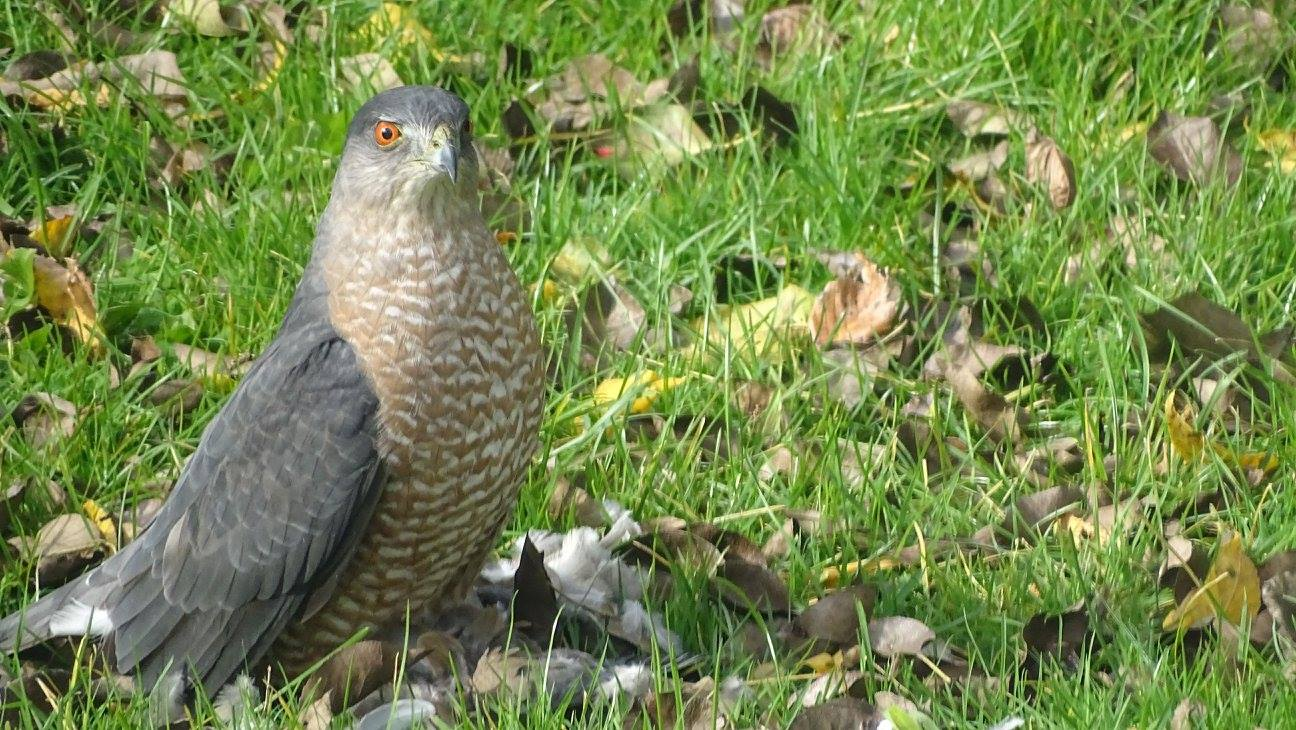
\includegraphics[width=.8\textwidth]{images/disapproving-bird}\footnote{Photo Credit: Danielle Guerard}
  \end{center}
\end{frame}
%%%%%%%%%%%%%%%%%%%%%%%%%%%%%%%%%%%%%%%%%%%%%%%%%%%%%%%%%%%%%%%%%%%%%%%%%%%%%%%%

%%%%%%%%%%%%%%%%%%%%%%%%%%%%%%%%%%%%%%%%%%%%%%%%%%%%%%%%%%%%%%%%%%%%%%%%%%%%%%%%
\begin{frame}[fragile]
  \frametitle{C++ atomics: Key Idea}
  
    An \emph{atomic operation} is indivisible.\\[1em]
    Other threads see state before or after the operation,
    nothing in between.
  
\end{frame}
%%%%%%%%%%%%%%%%%%%%%%%%%%%%%%%%%%%%%%%%%%%%%%%%%%%%%%%%%%%%%%%%%%%%%%%%%%%%%%%%

%%%%%%%%%%%%%%%%%%%%%%%%%%%%%%%%%%%%%%%%%%%%%%%%%%%%%%%%%%%%%%%%%%%%%%%%%%%%%%%%
\begin{frame}[fragile]
  \frametitle{Simplest: {\tt atomic\_flag}}
  
    Represents a boolean flag.\\[1em]
    \begin{lstlisting}[language=C]
#include <atomic>

atomic_flag f = ATOMIC_FLAG_INIT;
    \end{lstlisting}
  
\end{frame}
%%%%%%%%%%%%%%%%%%%%%%%%%%%%%%%%%%%%%%%%%%%%%%%%%%%%%%%%%%%%%%%%%%%%%%%%%%%%%%%%

%%%%%%%%%%%%%%%%%%%%%%%%%%%%%%%%%%%%%%%%%%%%%%%%%%%%%%%%%%%%%%%%%%%%%%%%%%%%%%%%
\begin{frame}[fragile]
  \frametitle{Operations on {\tt atomic\_flag}}
  
    Can clear, and can test-and-set:
    \begin{lstlisting}[language=C]
#include <atomic>

atomic_flag f = ATOMIC_FLAG_INIT;
int foo() {
  f.clear();
  if (f.test_and_set()) {
    // was true
  }
}
    \end{lstlisting}
    ~\\
    \begin{tabbing}
      {\tt test\_and\_set}: \= atomically sets to true, \\
      \> returns previous value.
    \end{tabbing}
    No assignment (=) operator.
  
\end{frame}
%%%%%%%%%%%%%%%%%%%%%%%%%%%%%%%%%%%%%%%%%%%%%%%%%%%%%%%%%%%%%%%%%%%%%%%%%%%%%%%%



\begin{frame}
\frametitle{Yet Another Rant About C++}

Although I guess in C++ you could define one if you wanted. 

This is kind of a dangerous thing about C++. 

If in C you see a line of code like \texttt{z = x + y;} you can have a pretty good idea about what it does and you can infer that there's some sort of natural meaning to the + operator there, like addition or concatenation. 

In C++, however, this same line of code tells you nothing unless you know...\\
\quad (1) the type of \texttt{x},\\
\quad (2) the type of \texttt{y}, and\\
\quad (3) how the \texttt{+} operator is defined on those two operands \textit{in that order}. 

But I'm digressing.


\end{frame}

%%%%%%%%%%%%%%%%%%%%%%%%%%%%%%%%%%%%%%%%%%%%%%%%%%%%%%%%%%%%%%%%%%%%%%%%%%%%%%%%
\begin{frame}[fragile]
  \frametitle{Using more general C++ atomics}


    Declaring them:
  
\begin{lstlisting}[language=C]
#include <atomic>

atomic<int> x;
\end{lstlisting}

Libary's implementation: \\
\hspace*{1em} on small types, lock-free operations;\\
\hspace*{1em} on large types, mutexes.
  

\end{frame}
%%%%%%%%%%%%%%%%%%%%%%%%%%%%%%%%%%%%%%%%%%%%%%%%%%%%%%%%%%%%%%%%%%%%%%%%%%%%%%%%

%%%%%%%%%%%%%%%%%%%%%%%%%%%%%%%%%%%%%%%%%%%%%%%%%%%%%%%%%%%%%%%%%%%%%%%%%%%%%%%%
\begin{frame}
  \frametitle{What to do with Atomics}

  
    \Large
    Kinds of operations:
    \begin{itemize}
    \item reads
    \item writes
    \item read-modify-write (RMW)
    \end{itemize}
  
\end{frame}
%%%%%%%%%%%%%%%%%%%%%%%%%%%%%%%%%%%%%%%%%%%%%%%%%%%%%%%%%%%%%%%%%%%%%%%%%%%%%%%%

%%%%%%%%%%%%%%%%%%%%%%%%%%%%%%%%%%%%%%%%%%%%%%%%%%%%%%%%%%%%%%%%%%%%%%%%%%%%%%%%
\begin{frame}[fragile]
  \frametitle{Reads and Writes}

  
    C++ has syntax to make these all transparent:
\begin{lstlisting}[language=C][language=C++]
#include <atomic>
#include <iostream>

std::atomic<int> ai;
int i;

int main() {
    ai = 4;
    i = ai;
    ai = i;
    std::cout << i;
}
\end{lstlisting}
Can also use {\tt i = ai.load()} and {\tt ai.store(i)}.
  
\end{frame}
%%%%%%%%%%%%%%%%%%%%%%%%%%%%%%%%%%%%%%%%%%%%%%%%%%%%%%%%%%%%%%%%%%%%%%%%%%%%%%%%

%%%%%%%%%%%%%%%%%%%%%%%%%%%%%%%%%%%%%%%%%%%%%%%%%%%%%%%%%%%%%%%%%%%%%%%%%%%%%%%%
\begin{frame}
  \frametitle{Read-Modify-Write (RMW)}

  
    Consider {\tt ai++}.\\[1em]
    This is really \\
    ~~~{\tt tmp = ai.read(); tmp++; ai.write(tmp); }\\[1em]
    Hardware can do that atomically.\\[1em]
    Other RMWs: {\tt +-, \&=, etc, compare-and-swap}\\[2em]

    {\small
      more info:\\ \url{http://preshing.com/20130618/atomic-vs-non-atomic-operations/}
      }
  
\end{frame}
%%%%%%%%%%%%%%%%%%%%%%%%%%%%%%%%%%%%%%%%%%%%%%%%%%%%%%%%%%%%%%%%%%%%%%%%%%%%%%%%


%%%%%%%%%%%%%%%%%%%%%%%%%%%%%%%%%%%%%%%%%%%%%%%%%%%%%%%%%%%%%%%%%%%%%%%%%%%%%%%%



\begin{frame}
\frametitle{Lock Freedom}

Suppose we'd like to operate in a world in which there are no locks. 

Research has gone into the idea of lock-free data structures. 

If you have a map and it will be shared between threads, the normal thing would be to protect access to the map with a mutex (lock). 

But what if the data structure was written in such a way that we didn't have to do that? 

That would be a lock-free data structure.

\end{frame}

\begin{frame}
\frametitle{Use Locks Wisely!}

For a great many situations, the normal locking and unlocking behaviour is sufficient.

We likely want to use it when we need to guarantee that progress is made. 

Or: when we really can't use locks (e.g., signal handler), or where a thread dying while holding a lock results in the whole system hanging.

\end{frame}

\begin{frame}
\frametitle{Non-Blocking Data Structure}

A non-blocking data structure is one where none of the operations can result in being blocked. 

In a language like Java there might be some concurrency-controlled data structures in which locking and unlocking is handled for you, but those can still be blocking. 

Lock-free data structures are always inherently non-blocking. 

A spin lock or busy-waiting approach is not lock free, because if the thread holding the lock is suspended then everyone else is stuck!

\end{frame}

\begin{frame}
\frametitle{Lock-Free Data Structure}
A lock-free data structure doesn't use any locks (duh) but there's also some implication that this is also thread-safe.

You can't make all your data structures lock-free ones by just deleting all the mutex code (sorry). 

Lock free also doesn't mean it's a free-for-all; there can be restrictions. 

For example, a queue that allows one thread to append to the end while another removes from the front, but not 2 removals at the same time.
\end{frame}



\begin{frame}
\frametitle{Lock-Free Data Structure}

The actual definition of lock-free is more formal. 

If any thread performing an operation gets suspended during the operation, then other threads accessing the data structure are still able to complete their tasks.

This is distinct from the idea of waiting, though; an operation might still have to wait its turn or might get restarted.

\end{frame}



\begin{frame}
\frametitle{Wait-Free Data Structures}

You might need wait-free data structures. 

This does not mean that nothing ever has to wait! 

It does mean that each thread trying to perform some operation will complete it within a bounded number of steps regardless of what any other threads do. 

This means that a compare-and-swap routine with infinite retries is not wait free, because a very unlucky thread could potentially take infinite tries...

The wait free data structures tend to be very complicated...

\end{frame}


\begin{frame}[fragile]
\frametitle{Example Lock-Free Algorithm}

\begin{lstlisting}[language=C]
void stack_push(stack* s, node* n) {
    node* head;
    do
    {
        head = s->head;
        n->next = head;
    }
    while ( !atomic_compare_exchange(s->head, head, n) );
} 
\end{lstlisting}

\end{frame}

\begin{frame}[fragile]
\frametitle{Example Wait-Free Algorithm}

\begin{lstlisting}[language=C]
void increment_reference_counter(rc_base* obj) {
    atomic_increment(obj->rc);
}

void decrement_reference_counter(rc_base* obj) {
    if (0 == atomic_decrement(obj->rc))
        delete obj;
} 
\end{lstlisting}

\end{frame}


\begin{frame}
\frametitle{To Lock Free, or Not to Lock Free}

Are lock-free programming techniques somehow better for performance? Maybe!

Lock free algorithms are about ensuring there is forward progress in the system and not really specifically about speed. 

A particular algorithm implementation might be faster under lock-free algorithms.

But often they are not. In fact, the lock free algorithms could be slower, in which case you use them because you must, not because it is particularly speedy.

\end{frame}


\end{document}

